% !TeX root = ../dissertation.tex

\chapter{Towards a Graphical User Interface for Uppex}

In order to make Uppex a more user-friendly tool for all types of users, initial steps were taken to develop an interface using Python and JavaScript.

\medskip

\noindent
\textbf{Requirements.} To be able to use the beta version of the tool, it is necessary to ensure that the following conditions are met: Python, the Java Virtual Machine (JVM), and Bash are installed, and Docker is available.

\medskip

\noindent
\textbf{Installation.} When the conditions above are met, the user can install this GUI by downloading and running the following Bash script:
\url{https://github.com/alexandre04032000/uppex-imitator/blob/Uppex-Imitator/interface.sh}. If the process runs successfully, the application will be available on port 8080 of the localhost.

\medskip

\noindent
\textbf{Running.} This interface allows users to choose between the desired model checker, specifically between Uppaal and IMITATOR. Once one of these options is selected, a menu is displayed (as shown in Figure \ref{fig:UI}), allowing the user to choose from the following options:

\begin{itemize}
    \item Validate the Model
    \item Run a Single Product
    \item Run All Products
    \item Change the Excel File
    \item Change .imi or .xml file
\end{itemize}

\begin{figure}[H]
    \centering
    \begin{minipage}{0.78\textwidth}
        \centering
        \begin{tikzpicture}
            \node[anchor=south west,inner sep=0] (image1) at (0,0) {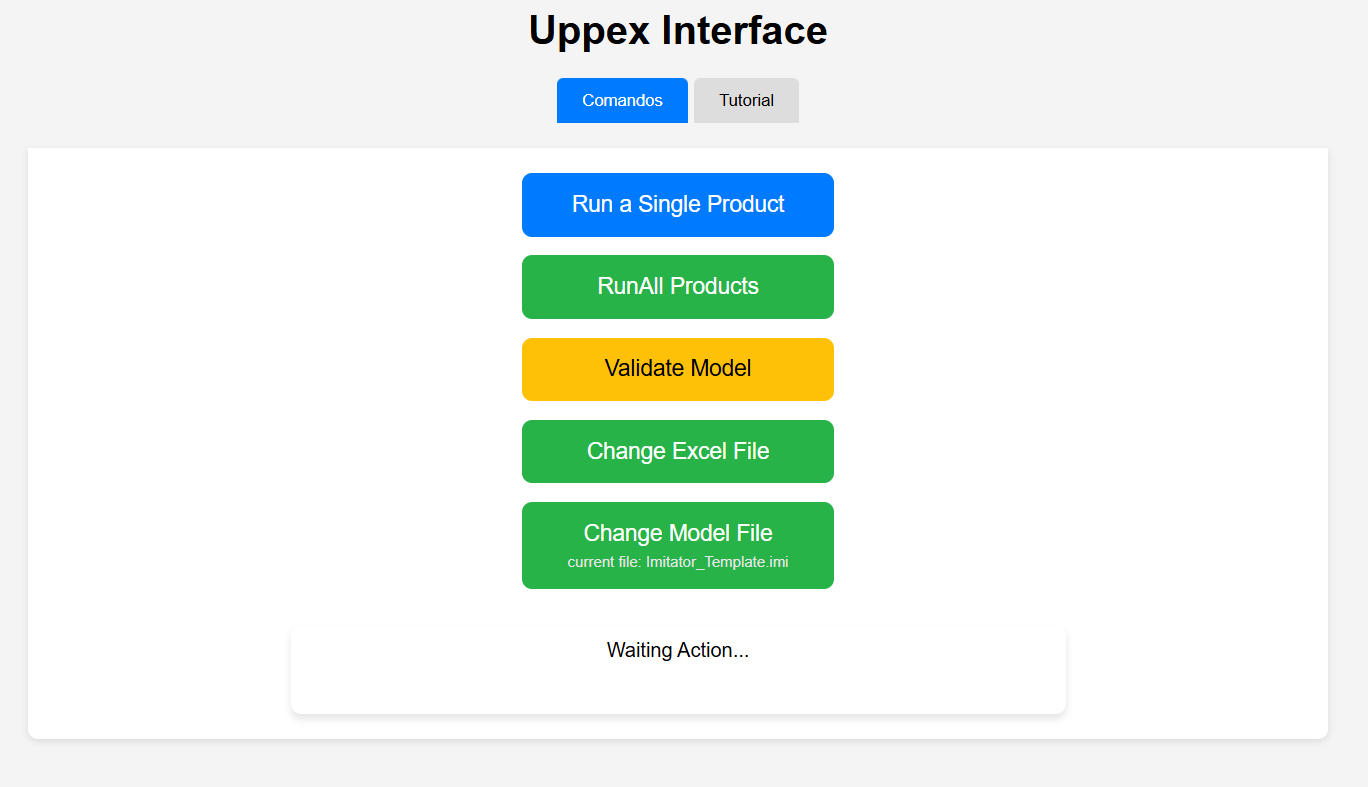
\includegraphics[width=\linewidth]{images/Interface.png}};
            \begin{scope}[x={(image1.south east)},y={(image1.north west)}]
                \draw[black, thick] (0,0) rectangle (1,1); % coordenadas normalizadas
            \end{scope}
        \end{tikzpicture}
        \caption{Uppex Interface Menu}
        \label{fig:UI}
    \end{minipage}
\end{figure}

It should be emphasized that, depending on the choice between Uppaal or Imitator in the menu shown in Figure \ref{fig:UI}, the extension of the file to be selected is already known in the last option, which also helps to identify which file is being read. There is also a separate tab called Tutorial which, as the name suggests, guides the user in interacting with the tool.



